\section{Results}\label{results}

In this section, we present our results on how velocity structure functions (VSFs) reflect the distribution of turbulent power within molecular clouds.

\subsection{Examples}\label{results:examples}

Fig.~\ref{pic:results:vsf_example} shows three examples of VSFs, (a) cloud \texttt{M4} at $t$~=~1.2~Myr after self-gravity has been activated in the simulations, (b) \texttt{M3} at $t$~=~3.5~Myr, and (c) \texttt{M3} at $t$~=~4.0~Myr.
All plots show the \textbf{density-weighted} VSFs of orders $p$~=~1--3.
The solid lines show the fitted power-law relations as given in Eq.~(\ref{equ:method:fitting}).

\begin{figure*}[!htb]
	\centering
	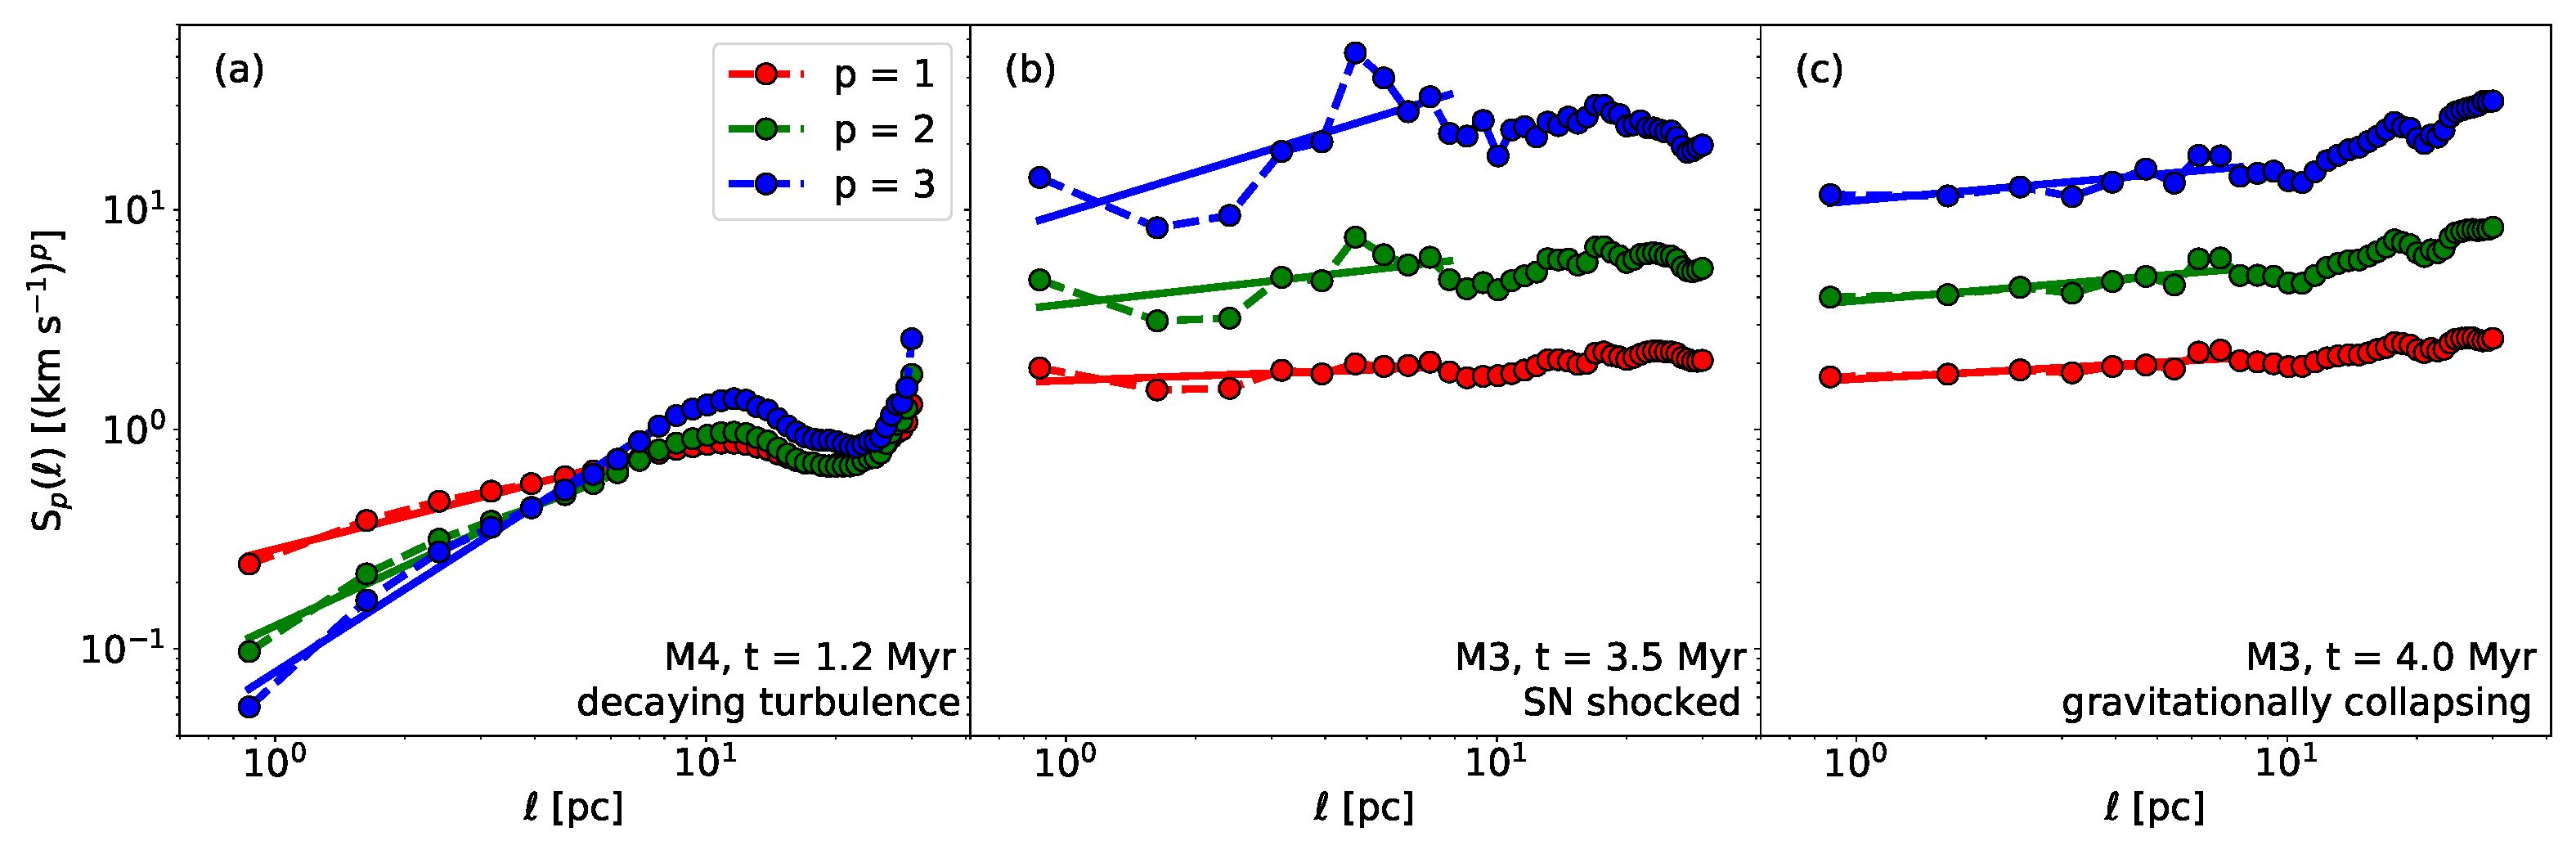
\includegraphics[width=\textwidth]{vsf_example.pdf}
    \caption{Examples of velocity structure functions as function of the lag scale, $\ell$, and order, $p$. 
    	The dots (connected by dashed lines) 
%mm illustrate the measured values based on the simulation data. 
    show the values computed from the simulation.
        The solid lines represent the power-law relations fitted to the respective structure functions.
	}
    \label{pic:results:vsf_example}
\end{figure*}

The examples demonstrate that, in general, the measured VSFs cannot be described by a single power-law relation over the entire range of $\ell$.
Instead they are composed of roughly three different regimes: 
one at small scales at $\ell \lesssim$~3~pc, a second one within 3~pc~$\lesssim \ell \lesssim$~10--15~pc, and the last one at large scales with $\ell >$~15~pc.
\textbf{We find that} only the small and intermediate ranges may be represented by a common power-law relation.
On larger scales, one observes a local minimum before the VSFs either increase or stagnate.
The location of the minimum coincides with the equivalent radius of the cloud, the radius a cloud of given mass would have if it would be a sphere.
\mm{[this is a pretty big claim to make based on one example. Can you make a plot showing the minimum location vs the equivalent radius for all three clouds for several times?  Otherwise, I'd consider cutting it.]}
Thus, in this context the VSF is an accurate tool to measure the size of a molecular cloud.
On smaller scales, which correspond to individual clumps and cores, one sees significant differences.

The examples in Fig.~\ref{pic:results:vsf_example} illustrate how VSFs react to different scenarios that affect the turbulent structure of the entire clouds. 
\textbf{Fig.~\ref{pic:results:vsf_example}(a) shows the case where turbulence is driven on large scales and naturally decays towards smaller scales.
This is the most common behavior seen in all three MCs within the first $\sim$1.5~Myr of the simulations.}
During this interval of time the clouds experience the effect of self-gravity for the first time in their evolution and need to adjust to this new condition.
Until this is the case, their VSFs are dominated by the freely cascading turbulence that previously dominated the kinetic structure of the clouds.
Furthermore, this implies that we can only reliably examine turbulence within the simulations after 1.5~Myr and carefully need to take this into account in the further discussion \citep[see][]{IbanezMejia2017,Seifried2017b}.

The other examples represent the clouds at later stages of their evolution when the VSFs are dominated by sources that drive the \textbf{low} within the clouds in a more extreme way.
Fig.~\ref{pic:results:vsf_example}(b) shows the VSF of \texttt{M3} at a time when the cloud has just been hit by a SN shock front. 
One clearly sees how the amplitude of the VSFs is increased by one to two orders of magnitudes compared to the previous example.
Especially the power \textbf{at small scales ($\ell \lesssim$ few parsecs) is highly amplified as a result of the shock, while it also reduces} the equivalent radius of the cloud.
\mm{[is that first minimum the thickness of the post-shock region, or the equivalent radius of the cloud?  I'd bet that it's the former.]}
Despite the increase of turbulent power at small scales, a large amount of energy is injected at large scales, as well.
All this results in a \textbf{shallower slope of the VSF}.
However, the effect of SN shocks last for only a short period of time (see below).

The last example, Fig.~\ref{pic:results:vsf_example}(c), demonstrates the imprint of gravitational contraction.
Here, the VSF is almost flat, or even slightly increasing towards smaller separation scales. 
This kind of profile is typical for gas that is self-gravitationally contracting \citep{Boneberg2015,Burkhart2015} since gas moves into the inner regions of the cloud, reducing the average lag distances, but not necessarily the relative velocities.
The latter may even be accelerated by the infall.
As a consequence, large amounts of kinetic energy are transferred to smaller scales which flattens the corresponding VSF.



\subsection{Time Evolution}\label{results:normal}

Fig.~\ref{pic:results:zeta_all}a plots the time evolution of $\zeta$ obtained for all three clouds.
The figure shows several interesting features.
First, initially, at $t$~=~0~Myr, all calculated values of $\zeta$ are above the predicted values (see Eqs.~(\ref{equ:method:she}) and~(\ref{equ:method:boldyrev})).
This means that the turbulence within the clouds is highly supersonic before the gas begins to react to the activation of self-gravity.
Second, all $\zeta$ decrease with time as the clouds gravitationally collapse.
\textbf{This gravitational collapse causes gas around the collapsing centers to accelerate, increasing the relative velocities at small scales. This process leads to the flattening of the exponent of the structure function, $\zeta$, as a function of time. }
Third, occasionally one observes bumps and dips in all orders of VSFs (e.g., \texttt{M3} or \texttt{M8} around $t$~=~1.7~Myr). 
These features only last for short periods of time (up to 0.6~Myr), but set in quasi-instantly and represent a complete relocation of the turbulent power particularly on large scales. 

\begin{figure*}[!htb]
	\centering  
  
  \begin{subfigure}[c]{\textwidth}
      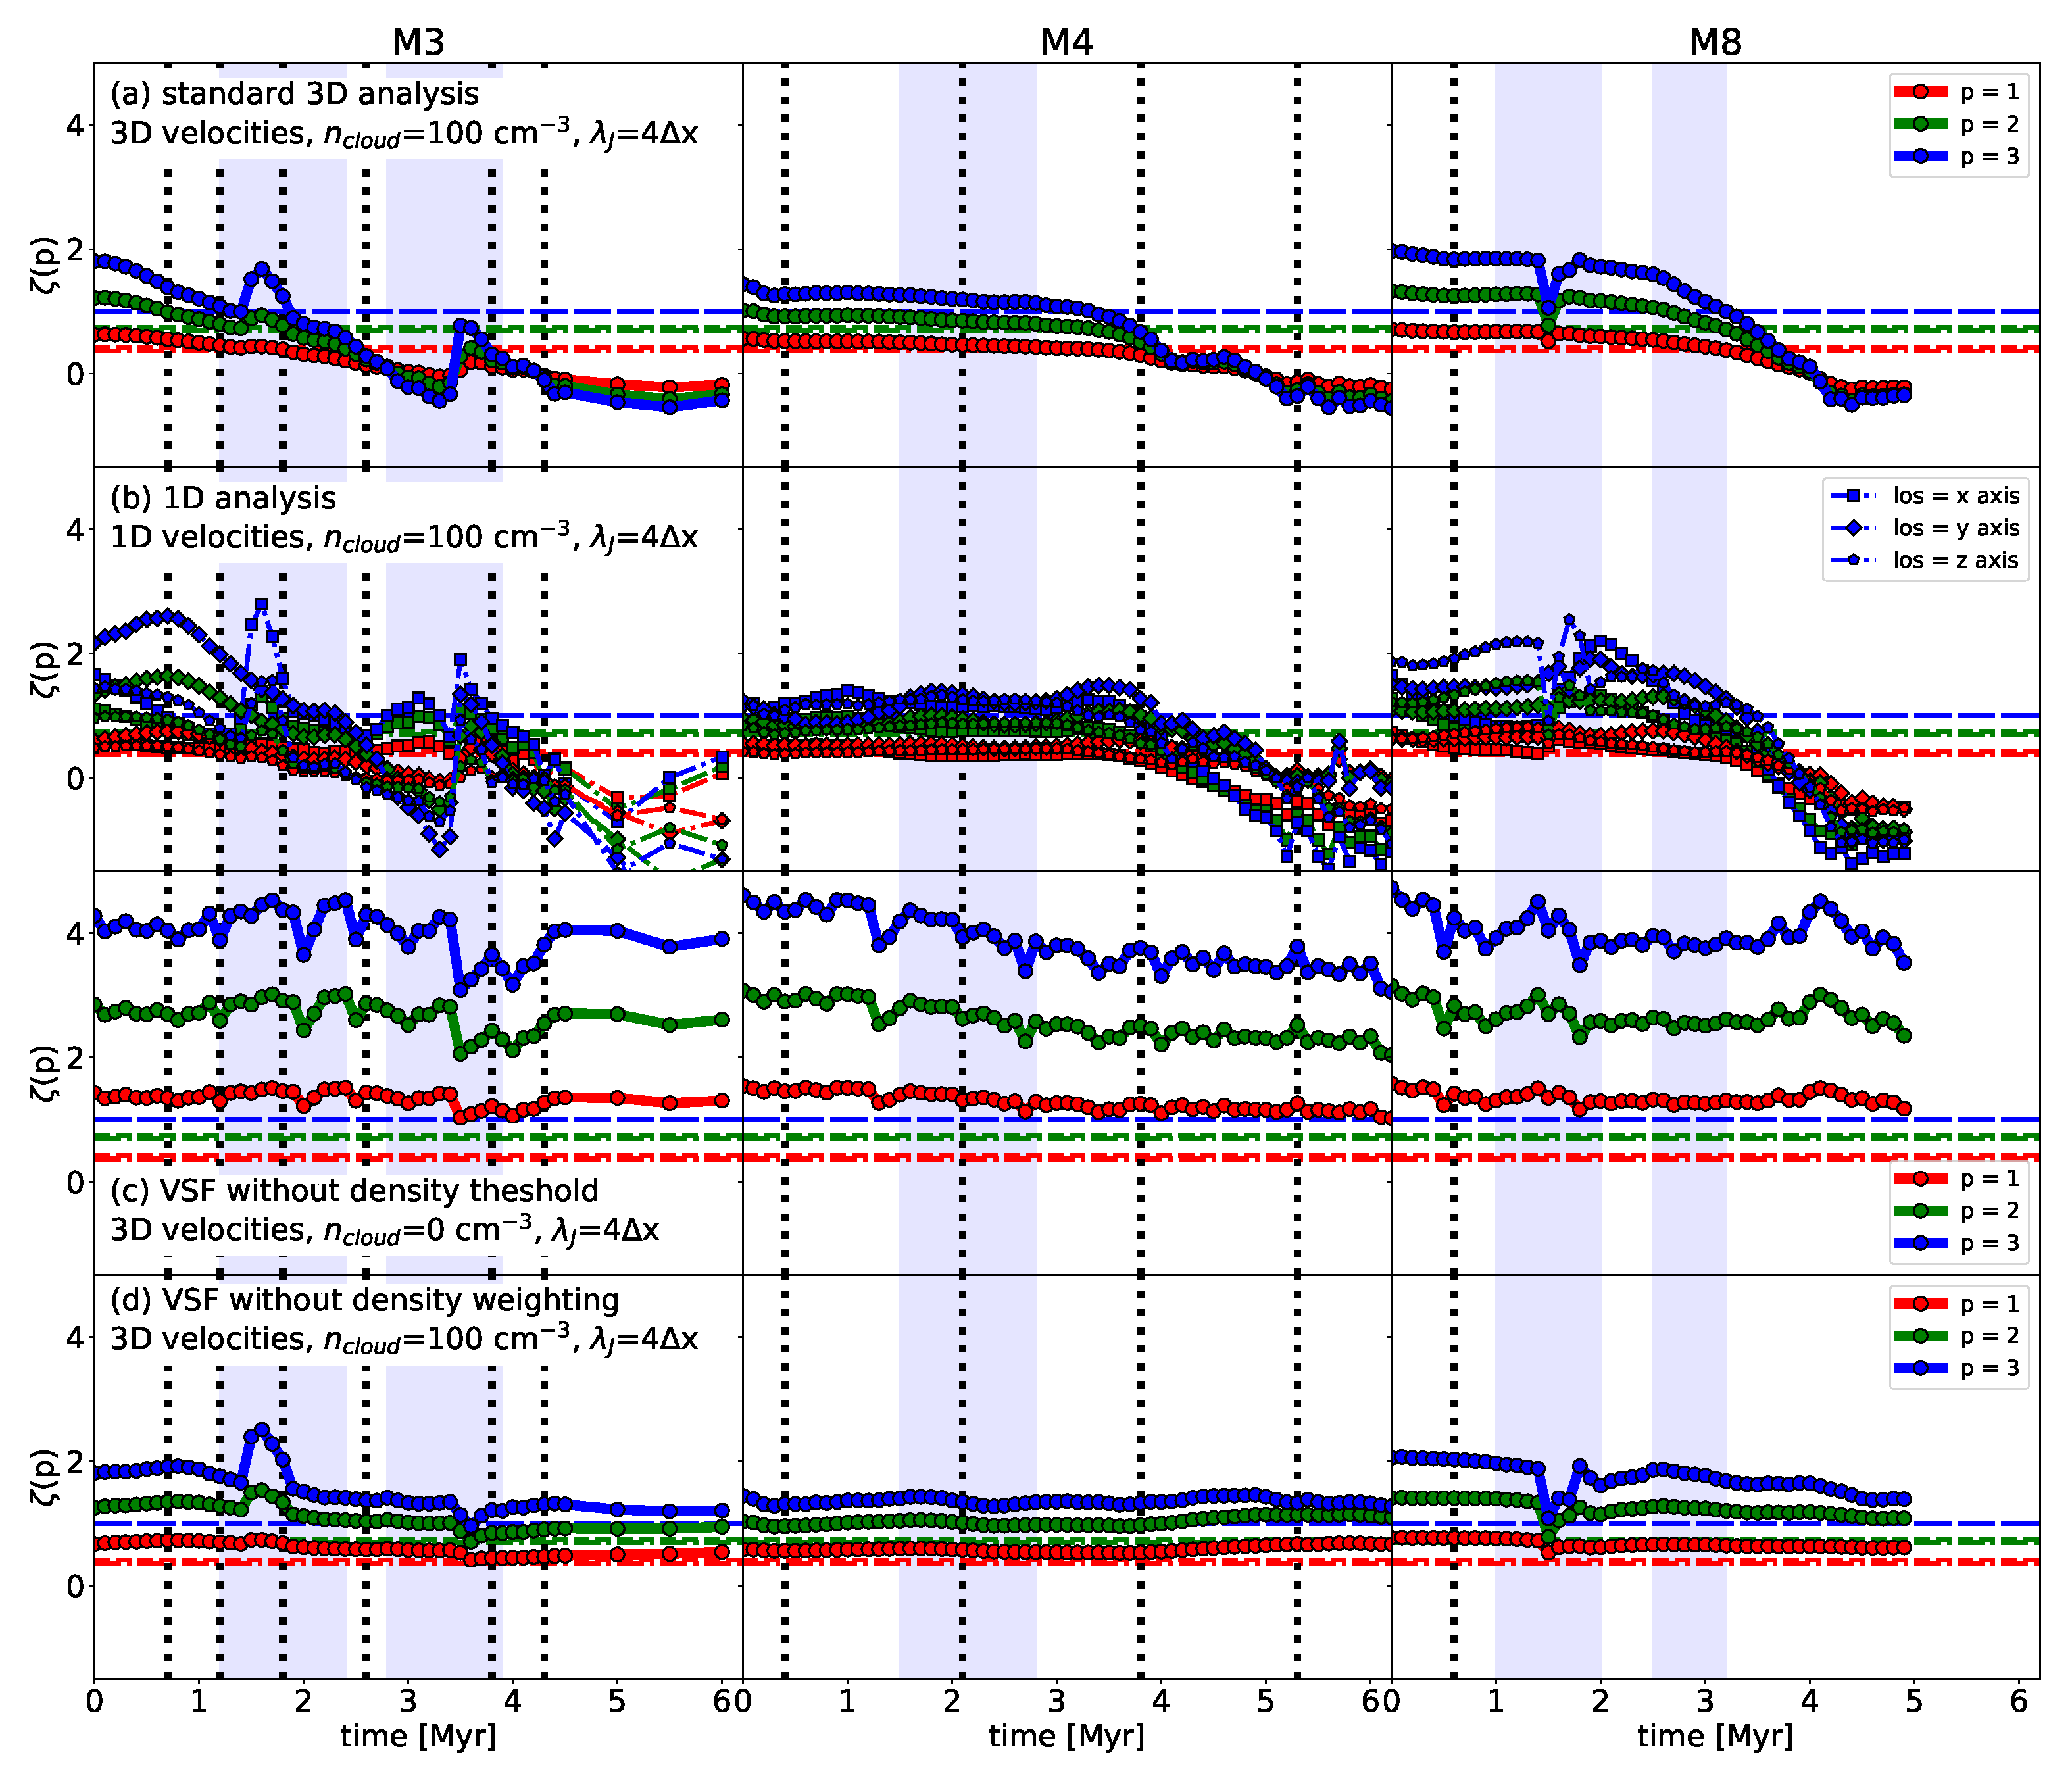
\includegraphics[width=\textwidth]{zeta_all_nojeans.pdf}
      \label{pic:results:zeta_all_nojeans}
  \end{subfigure}
  \begin{subfigure}[c]{\textwidth}
      \addtocounter{subfigure}{4}
      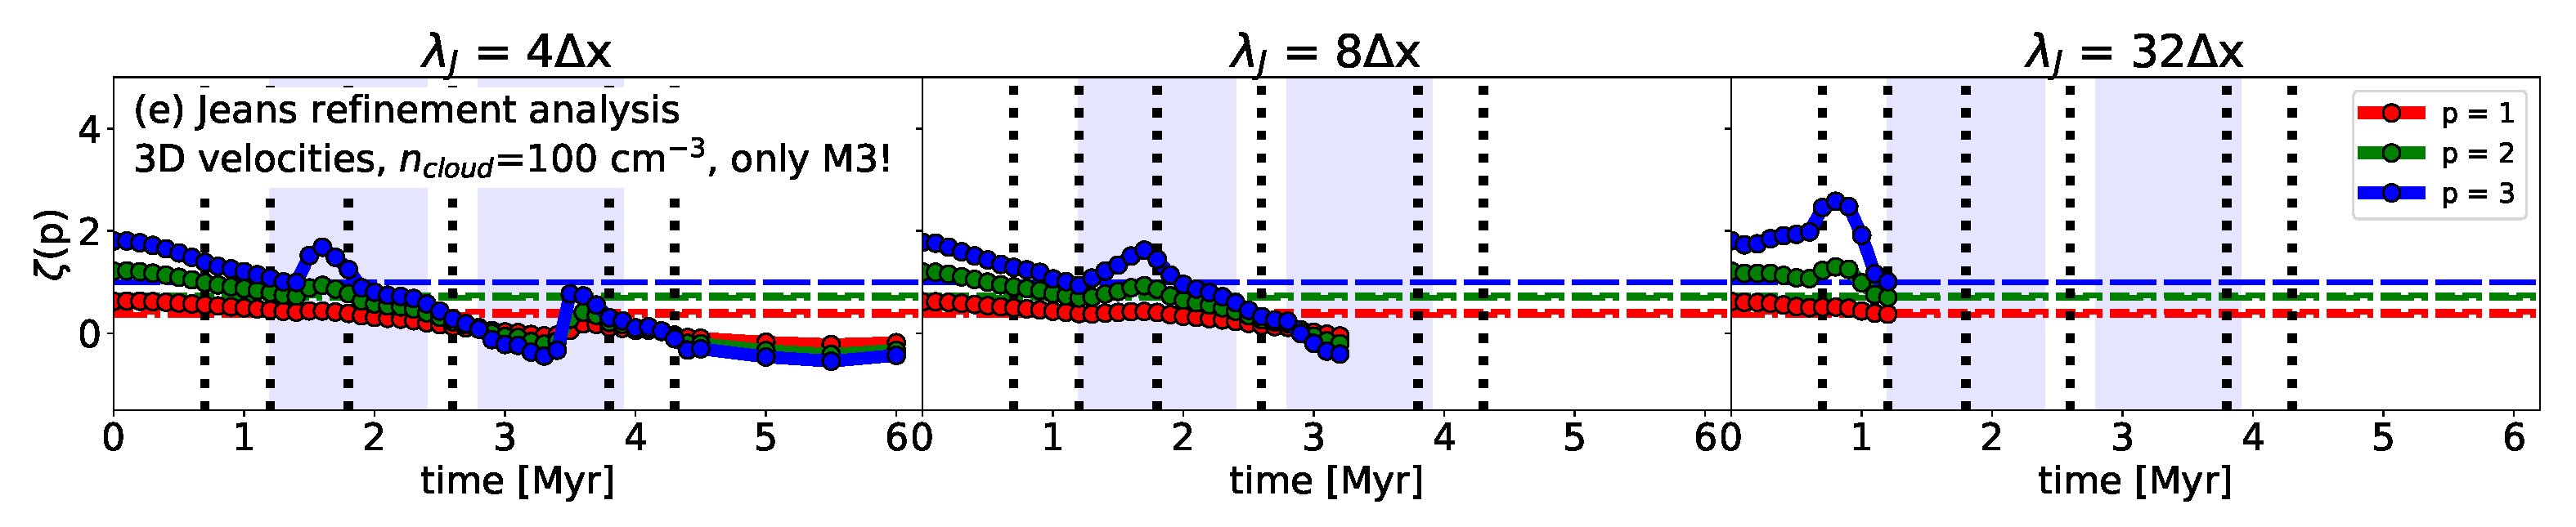
\includegraphics[width=\textwidth]{zeta_jeans.pdf}
      \label{pic:results:zeta_all_jeans}
  \end{subfigure}
  
  \caption{Time evolution of scaling exponent $\zeta$ of the $p^\mathrm{th}$ order VSF. The plots (a) -- (d) show the measurements for \texttt{M3} (\textit{left}), \texttt{M4} (\textit{middle}), and \texttt{M8} (\textit{right}), respectively. Thereby, (a) represents the standard analysis while the other rows illustrate the results of the test scenarios with input parameters adjusted as mentioned in the fiugures. The plots of (e) show the values of $\zeta$ measured within \texttt{M3} as function of the respective Jeans refinement level the cloud has been modelled with. The grey dotted vertical lines point to the times than a SN explodes within the vicinity of the corresponding cloud, while the blue areas indicate the time of enhanced mass accretion onto the clouds.}
	\label{pic:results:zeta_all}
\end{figure*}

\texttt{M8} seems to develop differently.
At the time the SN occurring at $t$~=~0.8~Myr hits the cloud the values of $\zeta$ do not rise, as they have done within the other two clouds, but instead they drop. 
After the shock all scaling exponents grow to levels that are slightly above the pre-shock values, before they slowly decrease again.

Fig.~\ref{pic:results:z_all}a shows the time evolution of the self-similarity parameter, $Z$, based on the model clouds. 
One sees that most of the time the measured values of $Z$ are in agreement or at least closely approaching the predicted values.
The peaks in the $Z$ (for example, in \texttt{M4} at $t$~=~4.1~Myr) occur at the times when the scaling exponents of the VSFs, $\zeta$, reach values close or below 0.
The decrease in $Z$ (for example, in \texttt{M3} around $t$~=~1.8~Myr), on the other hand, occur when SN shocks hit and heavily impact the clouds. 

\begin{figure*}[!htb]
	\centering  
  
  \begin{subfigure}[c]{\textwidth}
      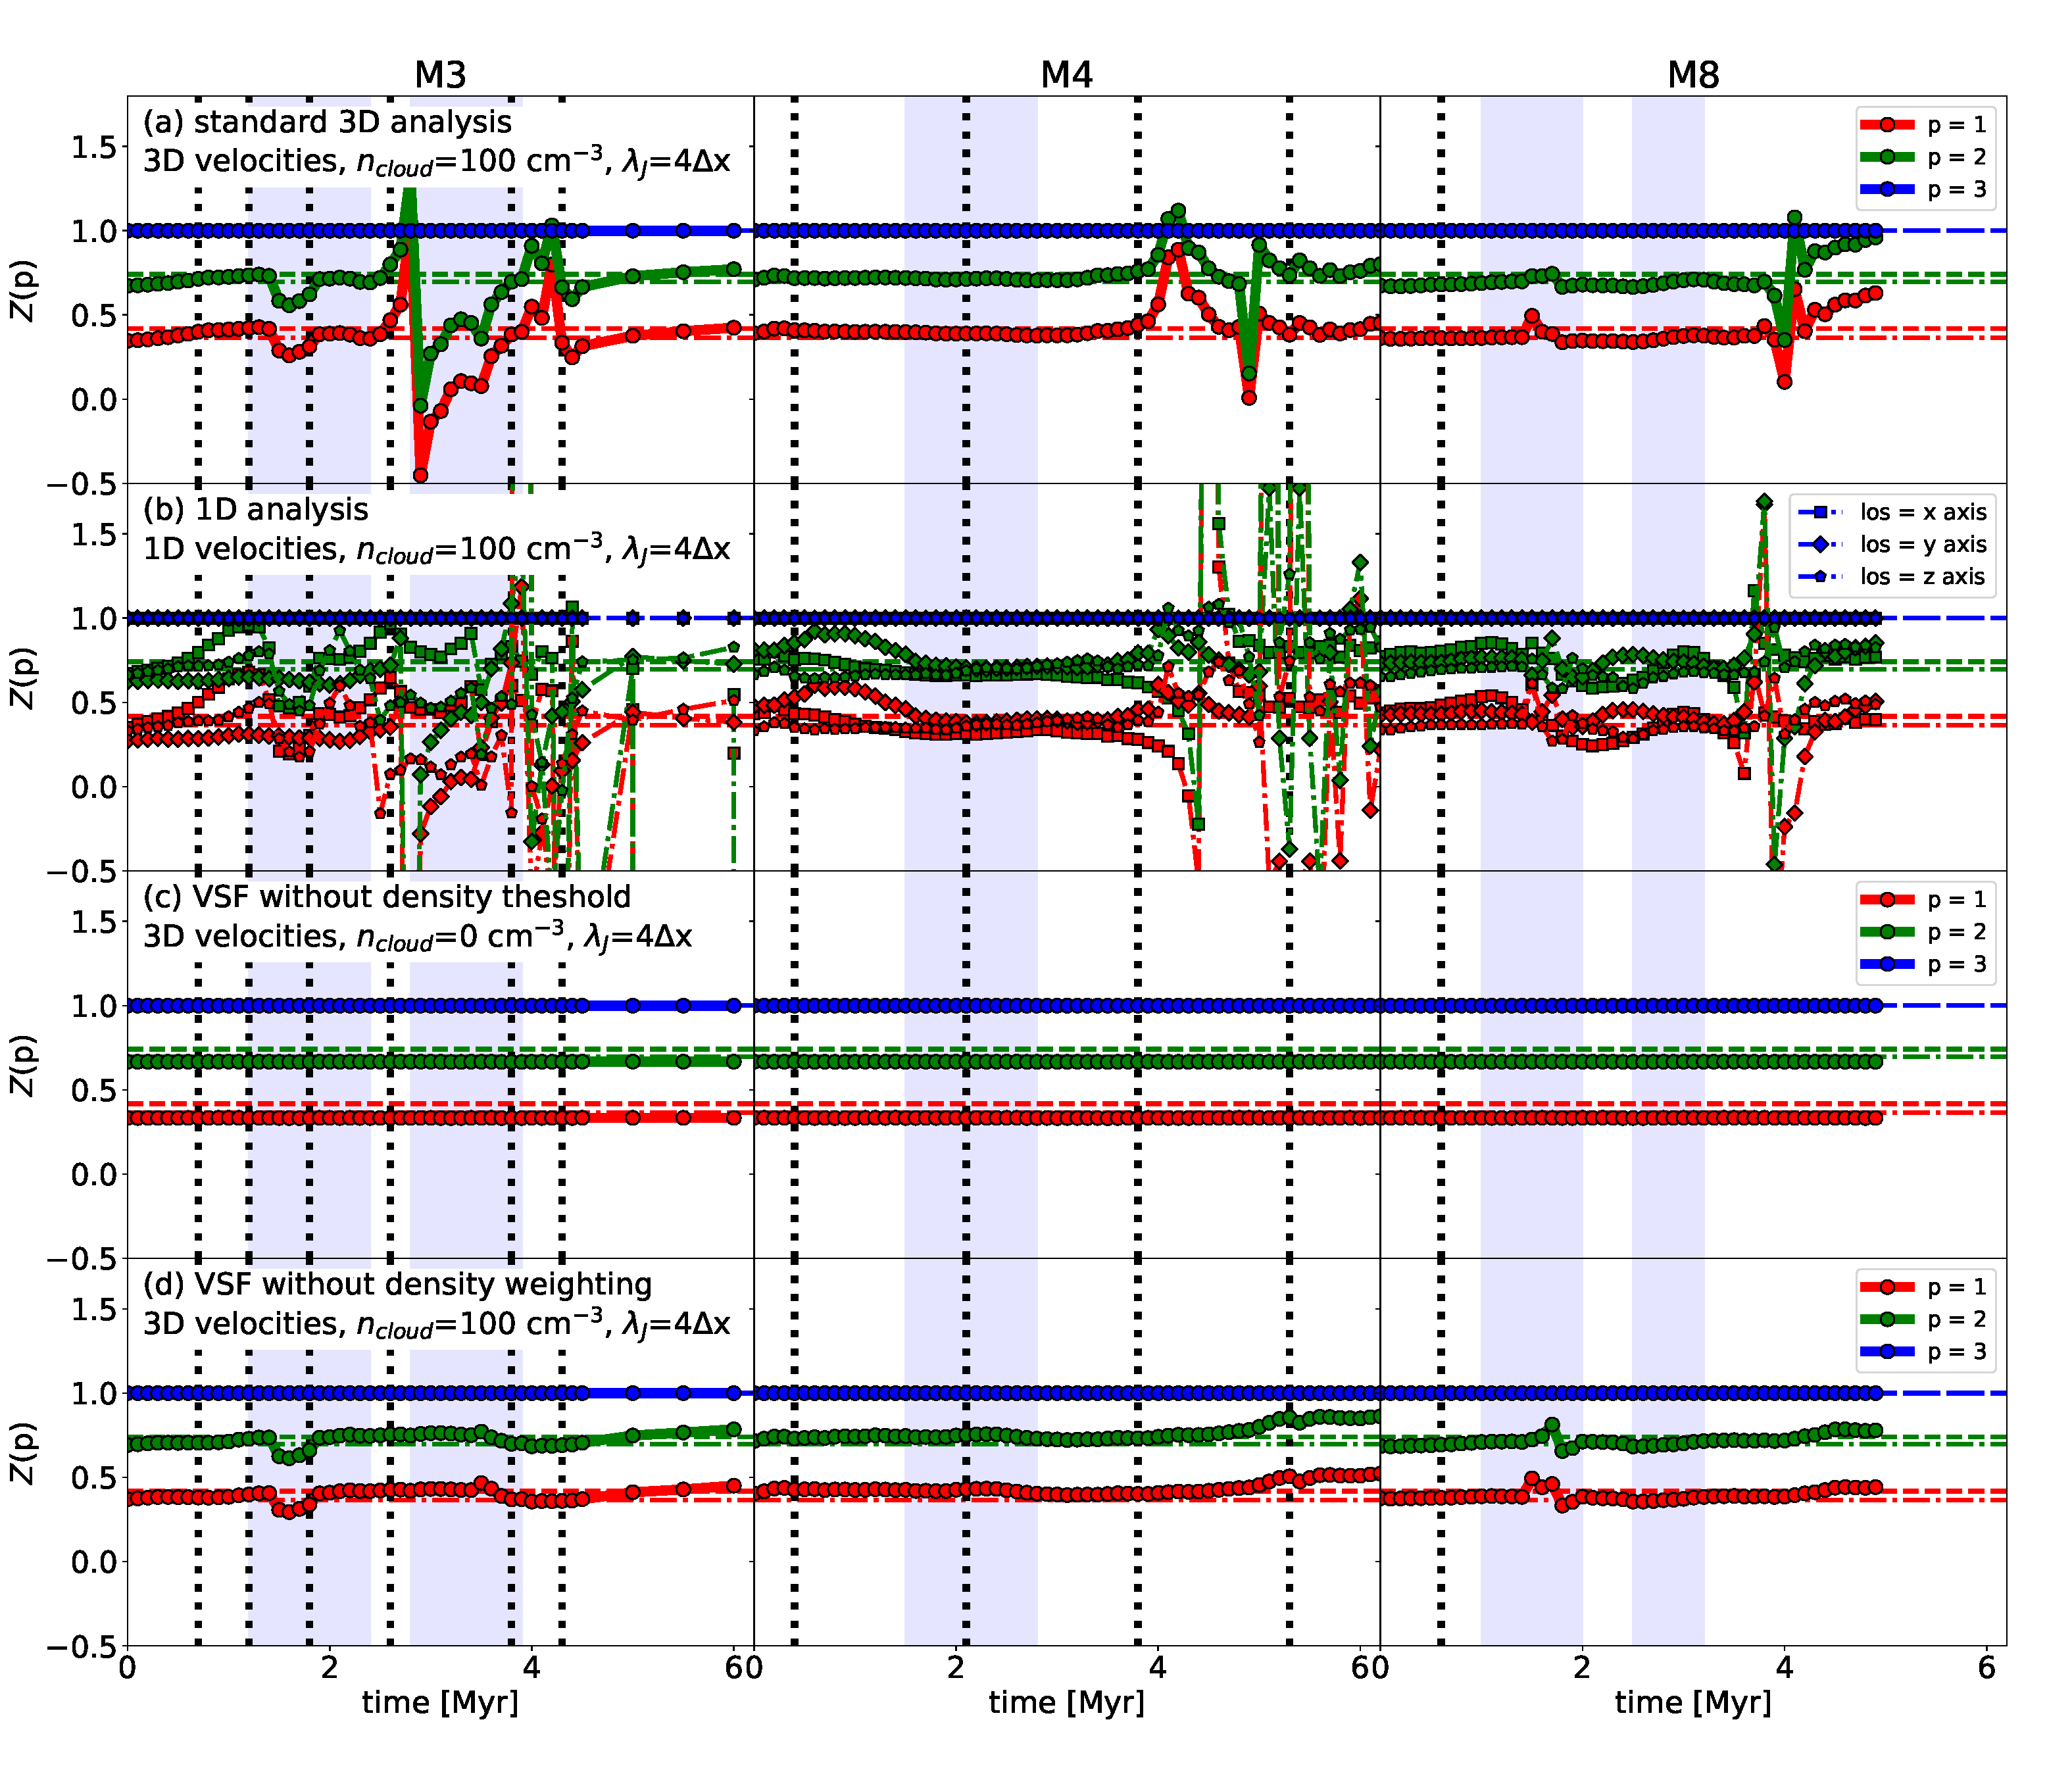
\includegraphics[width=\textwidth]{z_all_nojeans.pdf}
      \label{pic:results:z_all_nojeans}
  \end{subfigure}
  
  \begin{subfigure}[c]{\textwidth}
      \addtocounter{subfigure}{4}
      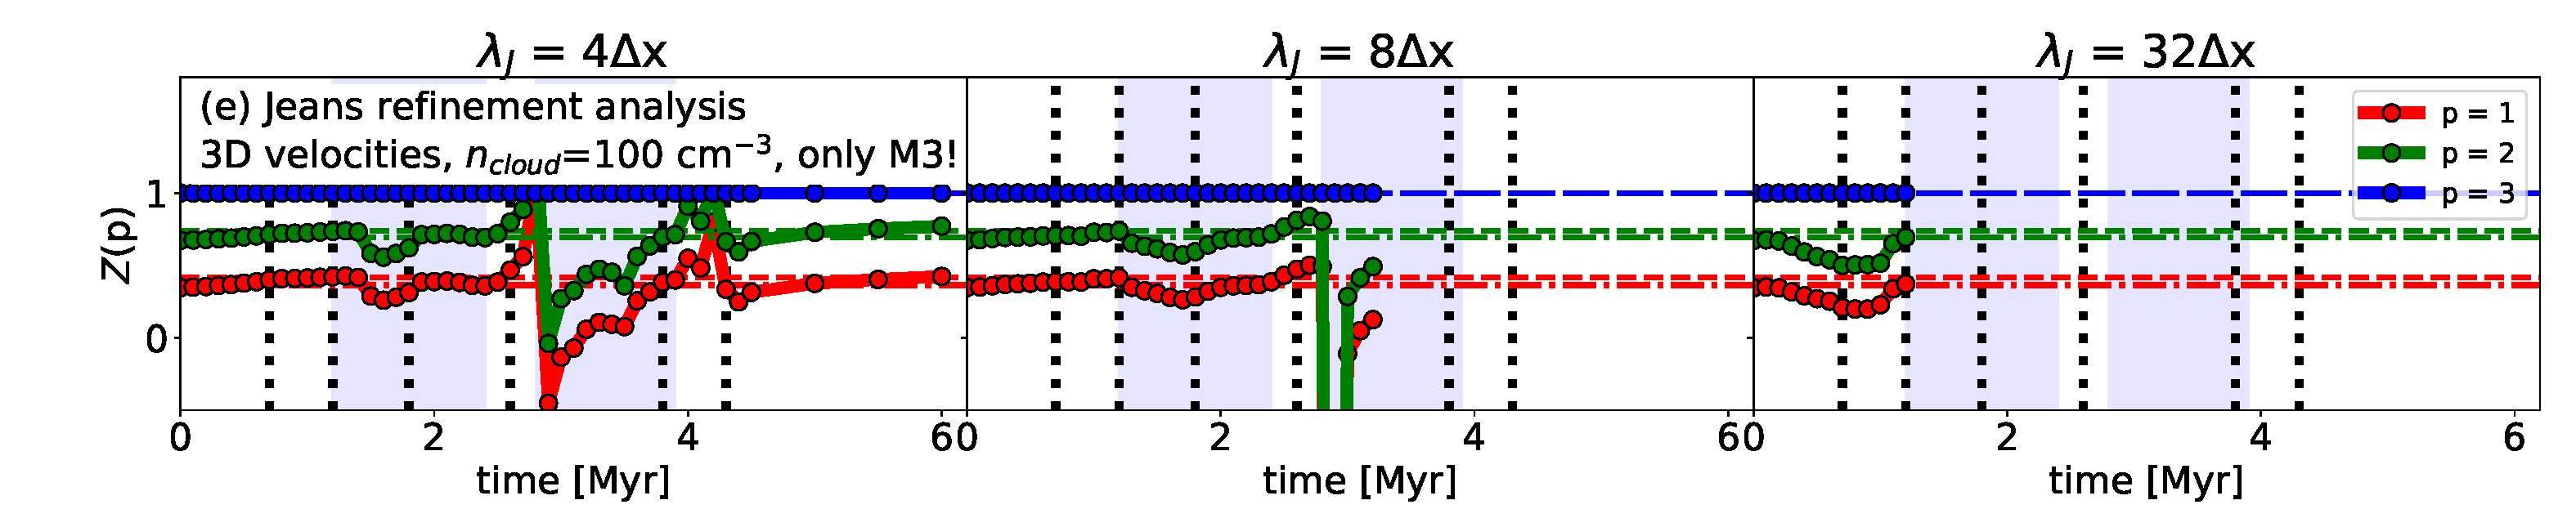
\includegraphics[width=\textwidth]{z_jeans.pdf}
      \label{pic:results:z_all_jeans}
  \end{subfigure}
  
  \caption{Like Fig.~\ref{pic:results:zeta_all}, but for the measured self-similarity parameter $Z = \zeta(p) / \zeta(3)$ of the $p^\mathrm{th}$ order VSF. The coloured horizontal lines show the predicted values by \citet{She1994} (dash-dotted lines) and \citet{Boldyrev2002} (dashed lines).}
	\label{pic:results:z_all}
\end{figure*}

In the following of this section, we will present how VSFs react to variety of setups that are typically assumed in comparable studies.
We will compare the findings with the results we have obtained with our original setup.
In Sect.~\ref{discussion}, we will discuss and interpret these results in more details.


\subsection{Comparison to Line-of-Sight Velocities}\label{results:1d}

Previously, we have seen how the VSF behaves and evolves within the clouds.
By doing so, we derived the relative velocities based on the 3D velocity vectors that we read out from the simulations.
Yet, this method is rather not applicable for many other studies. 
It is either computational expensive or not possible as observations generally only provide the velocity component along the line-of-sight (los).
Thus, in this subsection we investigate how VSFs derived from 1D relative velocities compare to the 3D VSFs presented before.
Thereby, we define the 1D VSF as follows:
\begin{equation}
	\mathit{S}_p^\mathrm{1D} (\ell) = \frac{\langle \, \rho(\vec{x}) \rho(\vec{x}+\vec{\ell}) \, |\Delta \vec{v} \cdot \vec{e}_i|^p  \, \rangle}{\langle  \, \rho(\vec{x}) \rho(\vec{x}+\vec{\ell}) \, \rangle} ,
    \label{equ:results:def_vsf_1d}
\end{equation}
with $\vec{e}_i$ representing the unit vector along the $i$~=~x-, y-, or z-axis.
Figs.~\ref{pic:results:zeta_all}b and~\ref{pic:results:z_all}b show measured $\zeta$ and $Z$, respectively, derived based on Eq.~(\ref{equ:results:def_vsf_1d}). 
We see that, in most of the cases, all 1D VSFs agree well with each other, as well as with the corresponding 3D VSFs.
Yet, there are cases in which the 1D VSF evolves temporarily or completely differently than the 3D VSF.
For example, the 1D VSF along the x-axis in \texttt{M3} initially behaves like the corresponding 3D VSF, if though with lower absolute values of $\zeta$ (or higher values of $Z$).
However, within $t$~=~2.5--3.8~Myr the samples diverge. 
While the 3D based $\zeta$ cease further and switch signs, the $\zeta$ based on the 1D VSF along the x-axis show a local maximum before converging with the 3D $\zeta$ again. 



\subsection{The Effect of Density Thresholds}\label{results:densthres}

Another assumption that significantly influence the structure and evolution of VSFs is the (number) density threshold, $n_\mathrm{cloud}$, that is normally applied to filter out the cells that are part of the clouds.
In this paper, we assume a minimal number density of $n_\mathrm{cloud}~=$~100~cm$^{-3}$.
This means that, when focusing on the cloud-only gas, we only consider those cells with number densities $n \geq n_\mathrm{cloud}$.
We have chosen this threshold as it roughly corresponds to the density when CO becomes detectable.

However, \citetalias{IbanezMejia2017} show that there is usually no harsh increase in density between the ISM and the clouds. 
Instead, the gas becomes continuously denser towards the centres of mass within the clouds. 
Consequently, introducing a density threshold is a rather artificial, physically weakly motivated distinction between the clouds and the ISM.
Observationally, however, introducing a density (or intensity) threshold is unavoidable, be it due to technical limitations (e.g., sensibility of detector) or the nature of the underlying physical processes (for example, excitation rates, or critical density).
Therefore, it is important to study to which extend a density threshold influences the VSF and its evolution.

\textbf{Furthermore, this approach considers only $\leq$1.5\% of the cubes' volumes.
Removing the density threshold, by setting n$_\mathrm{cloud}$~=~0~cm$^{-3}$, would results in analysing the data of the entire data cubes.
As this would be too computational expensive for the test scenario we present here, we randomly choose a set of 5\% of the total number of cells as reference points and compute relative velocities to these cells only.
We emphasise that this does not mean that we only calculate the relative velocities between those 5\% of cells.
Rather this subsample of cells represent the starting vectors $\vec{x}$ to which the velocities of all other cells $\vec{x} + \vec{\ell}$ in the same cube are compared to.
This way we reduce the risk of ignoring or emphasising any spatial direction or angle.}

\textbf{Note that by choosing the starting points randomly we ensure that all parts of the cubes are considered. 
As a consequence, there is only a little likelihood (5\%~$\times$~1.5\%~=~0.075\%) that cells that are associated with the clouds are chosen.
Therefore, we emphasise that it is likely that the two subsamples (no density threshold and cloud-only) do not necessarily have a common subset of starting vectors.
Yet, as we here still calculate relative velocities to all other cells in the cube, and that includes all cells making up the clouds, the resulting VSFs of the n$_\mathrm{cloud}$~=~0~cm$^{-3}$ sample also consists of most of the information of the inner-cloud interactions.}

In Figs.~\ref{pic:results:zeta_all}c and~\ref{pic:results:z_all}c we show the measured values of $\zeta$ and $Z$, respectively, that are derived from the data cubes without introducing an density threshold, meaning $n_\mathrm{cloud}~=$~0~cm$^{-3}$.
This means that we now do not only calculate the relative velocities between cells that are part of the clouds' volume, but between cells within the entire 400$^3$ cell cut-outs that contain both the clouds and the ISM.
For our calculations we apply the same methods as described in Sect.~\ref{methods}. 
Yet, in order to reduce the computational effort we choose only a randomly positioned subset of 3,200,000 cells (=~5\% of the entire 400$^3$ cube) within the entire cubes as reference points, $\vec{x}$. 
As the clouds make up only a small fraction of the volume within the cubes ($\approx$1.5\%), this approach makes it more like to pick locations within the modelled ISM, rather than cells within the clouds. 
We emphasise that, by doing so, we only influence the choice of $\vec{x}$ in Eq.~(\ref{equ:method:def_vsf}), not $\vec{x+\ell}$ as we still compute the relative velocities relative to every other cell at 3D lag distance $\ell$ within the entire cube. 

Figs.~\ref{pic:results:zeta_all}c and~\ref{pic:results:z_all}c clearly illustrate that the measurements in the samples without density threshold completely differ from those with the density threshold.
Fig.~\ref{pic:results:zeta_all}c shows that the measured values of $\zeta$ are by far higher in the ISM than in the cloud-only sample.
Although we see a similar decline of $\zeta$ in \texttt{M4} and \texttt{M8} as the gas contracts under the influence of gravity in the vicinity of the clouds, $\zeta$ generally evolve differently here than what we have observed for the cloud-only matter.
E.g., the pronounced features that have reflected the interactions between the clouds' gas and shock waves are either not as significantly visible or not present at all.
We see a high rate of random fluctuations in the evolution of $\zeta$, as well.
Furthermore, contrary to all of our other test scenarios, we see here that all $Z$ are constant in time and within all clouds, with values slightly lower than those predicted by \citet{She1994} for filamentary flows.


\subsection{The Effect of Density Weighting}\label{results:densweight}

As mentioned in Sect.~\ref{methods:vsf}, Eq.~(\ref{equ:method:def_vsf}) represents the definition of the density-weighted VSF.
The density weighting is required for this study to account for obtaining the data from smooth density distributions on Eulerian grids, instead of using individual Lagrangian test particles (or eddies) as it is actually supposed to.
Thus, the question is: How the two approaches compare with each other?
There are a few studies that have targeted this question \citep[e.g.,][]{Benzi1993,Benzi2010,Gotoh2002,Schmidt2008}. 
However, all of them considered turbulent flows in sterile, homogeneous environments that are not comparable to our clouds.
Other studies, like \citet{Padoan2016a}, use both methods, but not on the same set of data. 

In this section, we investigate the influence of density weighting on VSFs by repeating the original analysis with the non-weighted VSF given by,
\begin{equation}
	\mathit{S}_p (\ell) = \langle \, |\Delta \vec{v}|^p  \, \rangle = \langle \, |\vec{v}(\vec{x}) - \vec{v}(\vec{x} + \vec{\ell})|^p  \, \rangle .
    \label{equ:results:def_vsf_no}
\end{equation}
Figs.~\ref{pic:results:zeta_all}d and~\ref{pic:results:z_all}d show the measured values of $\zeta$ and $Z$ derived from the non-weighted VSFs, respectively.

Comparing the weighted and non-weighted samples, we see the following:
The non-weighted $\zeta$ (Fig.~\ref{pic:results:zeta_all}d) and $Z$ (Fig.~\ref{pic:results:z_all}d) trace the interactions between the gas of the clouds and the SN shocks in the same way as we have seen it for the density-weighted VSF.
In \texttt{M3} and \texttt{M8} we also see that the values of $\zeta$ decrease as the clouds evolve, yet not as fast as they do in the density-weighted VSFs. 
The measurements in \texttt{M4}, however, are almost constant over time. 
In all the cases, the values of $\zeta$ never cease below 0.5; a behaviour that clearly differs from what we have observed in the density-weighted VSFs.

We observe a similar behaviour for measured $Z$. 
As before, they are almost constant over time and in good agreement with predicted values.
The only derivations we see compared to the previous results are caused by the interactions between the clouds and incoming SN shock fronts, with levels of disturbance that are similar to the measurements using density-weighted VSFs. 
However, the evolution of $Z$s is smoother as there is no sign inversion of $\zeta$.
This means that we do not have any strong peaks in $Z$ indicating the time when $\zeta(3)$ approaches 0, which happened when the majority of the turbulent power has been transferred to the small scales. 

Fig.~\ref{pic:results:comp_weighting} summarises the comparison of $\zeta$ (\textit{top}) and $Z$ (\textit{bottom}) measured with the density-weighted (\textit{abscissas}) and non-weighted VSFs (\textit{ordinates}) for all Jeans refinement levels \textbf{(meaning the granularity used for modelling the turbulent motions of the gas, see Sect.~\ref{results:refinement} for more details)}.
The figure clearly shows that the measurements only agree well for the highest refinement level with $\lambda~=~32\Delta x$.
However, we would need more data point to be sure that this correlation is indeed real.
At lower refinement level the measurements\textbf{, as those used for the standard analysis and all other test scenarios but the one presented in Sect.~\ref{results:refinement},} correlate less well with each other. 
The differences in the samples appear dominantly when the density-weighted $\zeta$ cease below $\approx$0.5, which is the global minimum for the non-weighted $\zeta$. 
This means that none of the $\zeta$ computed in all clouds and refinement levels with the non-weighted VSF is measured to be below 0.5. 

\begin{figure*}
	\centering
    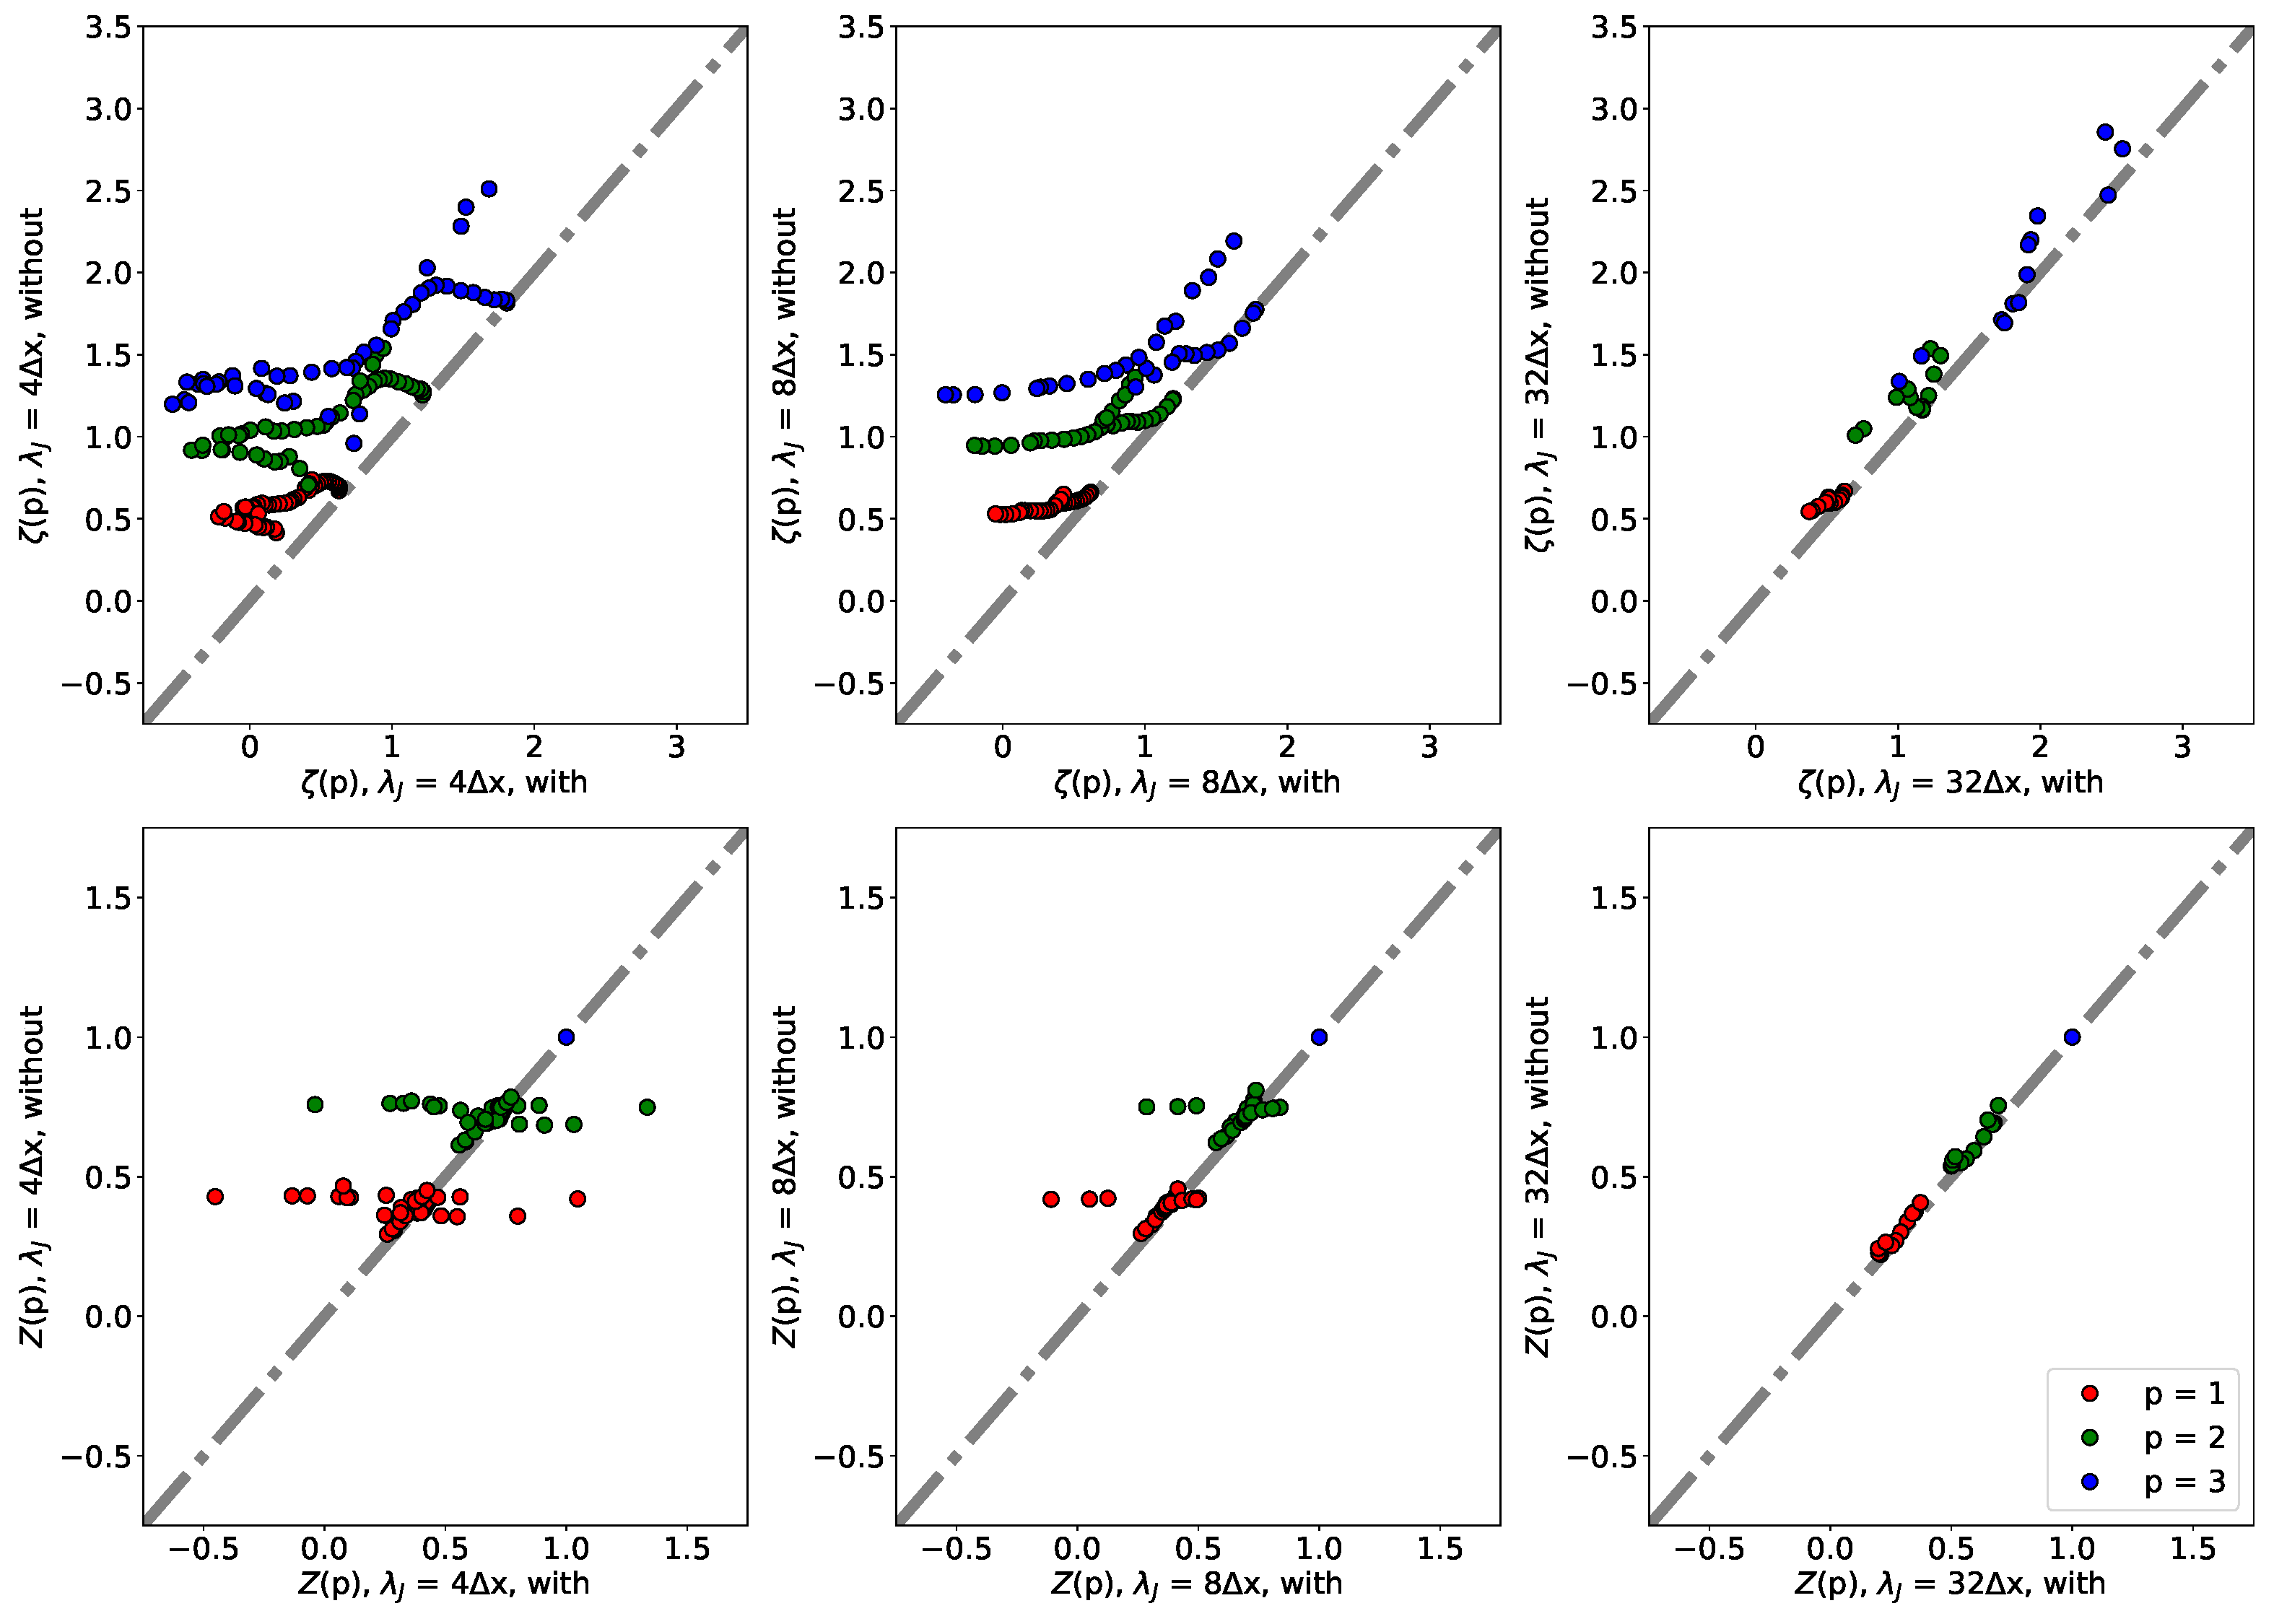
\includegraphics[width=\textwidth]{comp_weighting.pdf}
    \caption{ Comparison of $\zeta$ (\textit{top}) and $Z$ (\textit{bottom}) measured based on density-weighted VSFs (\textit{abscissas}) and non-weighted VSFs (\textit{ordinates}). }
    \label{pic:results:comp_weighting}
\end{figure*}




\subsection{The Effect of Jeans Length Refinement}\label{results:refinement}

The results we have discussed so far are based on simulation data as they have been presented in \citetalias{IbanezMejia2016} and \citetalias{IbanezMejia2017}.
Due to the huge computational expense the variety of physical and numerical processes (fluid dynamics, adaptive mesh refinement, supernovae, magnetic fields, radiative heating and cooling, and many more) within those simulations, though, have demanded some compromises.

One of these compromises has been the Jeans refinement criterion as part of the AMR mechanisms.
The authors have resolved local Jeans lengths by only four cells ($\lambda_J$~=~$4\Delta{}x$).
This is the minimal requirement for modelling self-gravitating gas in order to avoid artificial fragmentation \citep{Truelove1998}. 
Other studies, for example by \citet{Turk2012}, have shown that a significant higher refinement is needed to reliably resolve turbulent structures and flows on scales of individual cells.

In the appendix of \citetalias{IbanezMejia2017}, the authors examine the effect the number of cells used for the Jeans refinement has on the measured kinetic energy.
For this, they have rerun the simulations of \texttt{M3} twice; 
once with a refinement of eight cells per Jeans length ($\lambda_J$~=~$8\Delta{}x$) for the first 3~Myr after self-gravity was activated, and once with 32 cells per Jeans length ($\lambda_J$~=~$32\Delta{}x$) for the first megayear of the cloud's evolution.
The authors show that the $\lambda_J$~=~$32\Delta{}x$ simulations smoothly reveal the energy power spectrum on all scales already after this first megayear.
The other two setups do this, as well.
However, they need more time to overcome the resonances in the respective power spectra that originate from the previous resolution steps. 
This is why one can only then fully reliably trust the findings in this paper after the clouds have evolved for approximately 1.5~Myr \citep[see also][]{IbanezMejia2017,Seifried2017b}.

Furthermore, \citetalias{IbanezMejia2017} have calculated the difference in the cloud's total kinetic energy as function of time and refinement level.
They found that the $\lambda_J$~=~$4\Delta{}x$ simulations miss a significant amount of kinetic energy, namely up to 13\% compared to $\lambda_J$~=~$8\Delta{}x$ and 33\% compared to $\lambda_J$~=~$32\Delta{}x$.
However, they also observed that these differences peak around $t$~=~0.5~Myr and decrease afterwards, as the $\lambda_J$~=~$4\Delta{}x$ and $\lambda_J$~=~$8\Delta{}x$ simulations adjust to the new refinement levels.
This, of course, means that the results we have derived from the $\lambda_J$~=~$4\Delta{}x$ simulations always needs to be evaluated with respect to this lack of energy, although the clouds' dynamics is dominated by gravitational collapse.
It also means that the $\lambda_J$~=~$4\Delta{}x$ data become more reliable the longer the simulations have time to evolve.

In this section, we present how the level of Jeans refinement influences the behaviour of the VSFs.
In order to do so, we investigate the \texttt{M3} data of the $\lambda_J$~=~$8\Delta{}x$ and $\lambda_J$~=~$32\Delta{}x$ simulations in the same way as we have done with the $\lambda_J$~=~$4\Delta{}x$ data: measure the VSFs and analyse the time evolution of $\zeta$ and $Z$.
Figs.~\ref{pic:results:zeta_all}e and \ref{pic:results:z_all}e show the measure values of $\zeta$ and $Z$ for the $\lambda_J$~=~$8\Delta{}x$ and $\lambda_J$~=~$32\Delta{}x$.
In Fig.~\ref{pic:results:jeans_comp} we directly compare the measurements of all refinement levels relative to $\lambda_J$~=~$4\Delta{}x$.

$\lambda_J$~=~$8\Delta{}x$ shows the same behaviour as $\lambda_J$~=~$4\Delta{}x$ previously, with values in both samples being in good agreement as the top panel of Fig.~\ref{pic:results:jeans_comp} demonstrates. 
Over the entire observed time span, the measured values of $\zeta$ decreases as the VSF become flatter.
At the time the SNe interact with the cloud, the VSFs steeply increase forward larger scales, causing values of $\zeta$ (Fig.~\ref{pic:results:zeta_all}e).
Compared to the $\lambda_J$~=~$4\Delta{}x$ sample, the peak in $\zeta$ is smoother and last longer here, reflecting an impact time span of a bit less than 1~Myr.

This is observable in Fig.~\ref{pic:results:z_all}e where the sink of $Z$ due to the SN shock lasts longer than it has done in within the $\lambda_J$~=~$4\Delta{}x$ simulations. 
Besides this, the time evolution of $Z$ based on the $\lambda_J$~=~$8\Delta{}x$ simulations is as sensitive to the turbulence-related events as it has been for $\lambda_J$~=~$4\Delta{}x$.
The divergence which is produced when gravity has transferred the majority of power to smaller scales occurs at the same time. 
Thereby, the depth of the sink is a numerical artefact caused by $\zeta(3)$ being equal or close to 0 at this very time step. 

The picture changes when we analyse the VSFs based on the $\lambda_J$~=~$32\Delta{}x$ runs (Figs.~\ref{pic:results:zeta_all}e,~\ref{pic:results:z_all}e, and~\ref{pic:results:jeans_comp}).
Here one sees that the measured values of both $\zeta$ (Fig.~\ref{pic:results:zeta_all}e) and $Z$ (Fig.~\ref{pic:results:z_all}e) are similar to those for $\lambda_J$~=~$4\Delta{}x$ for the first 0.2~Myr.
After this short period, though, the evolutions of $\zeta$ diverge. 
While $\zeta(1)$ and $\zeta(2)$ continue to decrease in similar, but on lower rates compared to $\lambda_J$~=~$4\Delta{}x$, $\zeta(3)$ increases until it peaks at $t$~=~0.8~Myr and falls steeply down again.
This divergence has notable impact on the evolution of $Z$, as well. 
The bottom panel of Fig.~\ref{pic:results:jeans_comp} illustrates the different evolutions of measured $\zeta$ and $Z$ in the two samples of simulations more clearly.
One sees that the differences between the samples follow the same pattern for all orders of $p$.
The differences, though, increases with the order:
While the values for $\zeta(1)$ are still in good agreement, the measured values of $\zeta(2)$ and $\zeta(3)$ for $\lambda_J$~=~$32\Delta{}x$ are 40\% and 100\% higher than those measured for $\lambda_J$~=~$4\Delta{}x$, respectively.
Consequently, this causes differences in $Z(p)$ within 30--52\% between the simulations.

\begin{figure*}
	\centering
    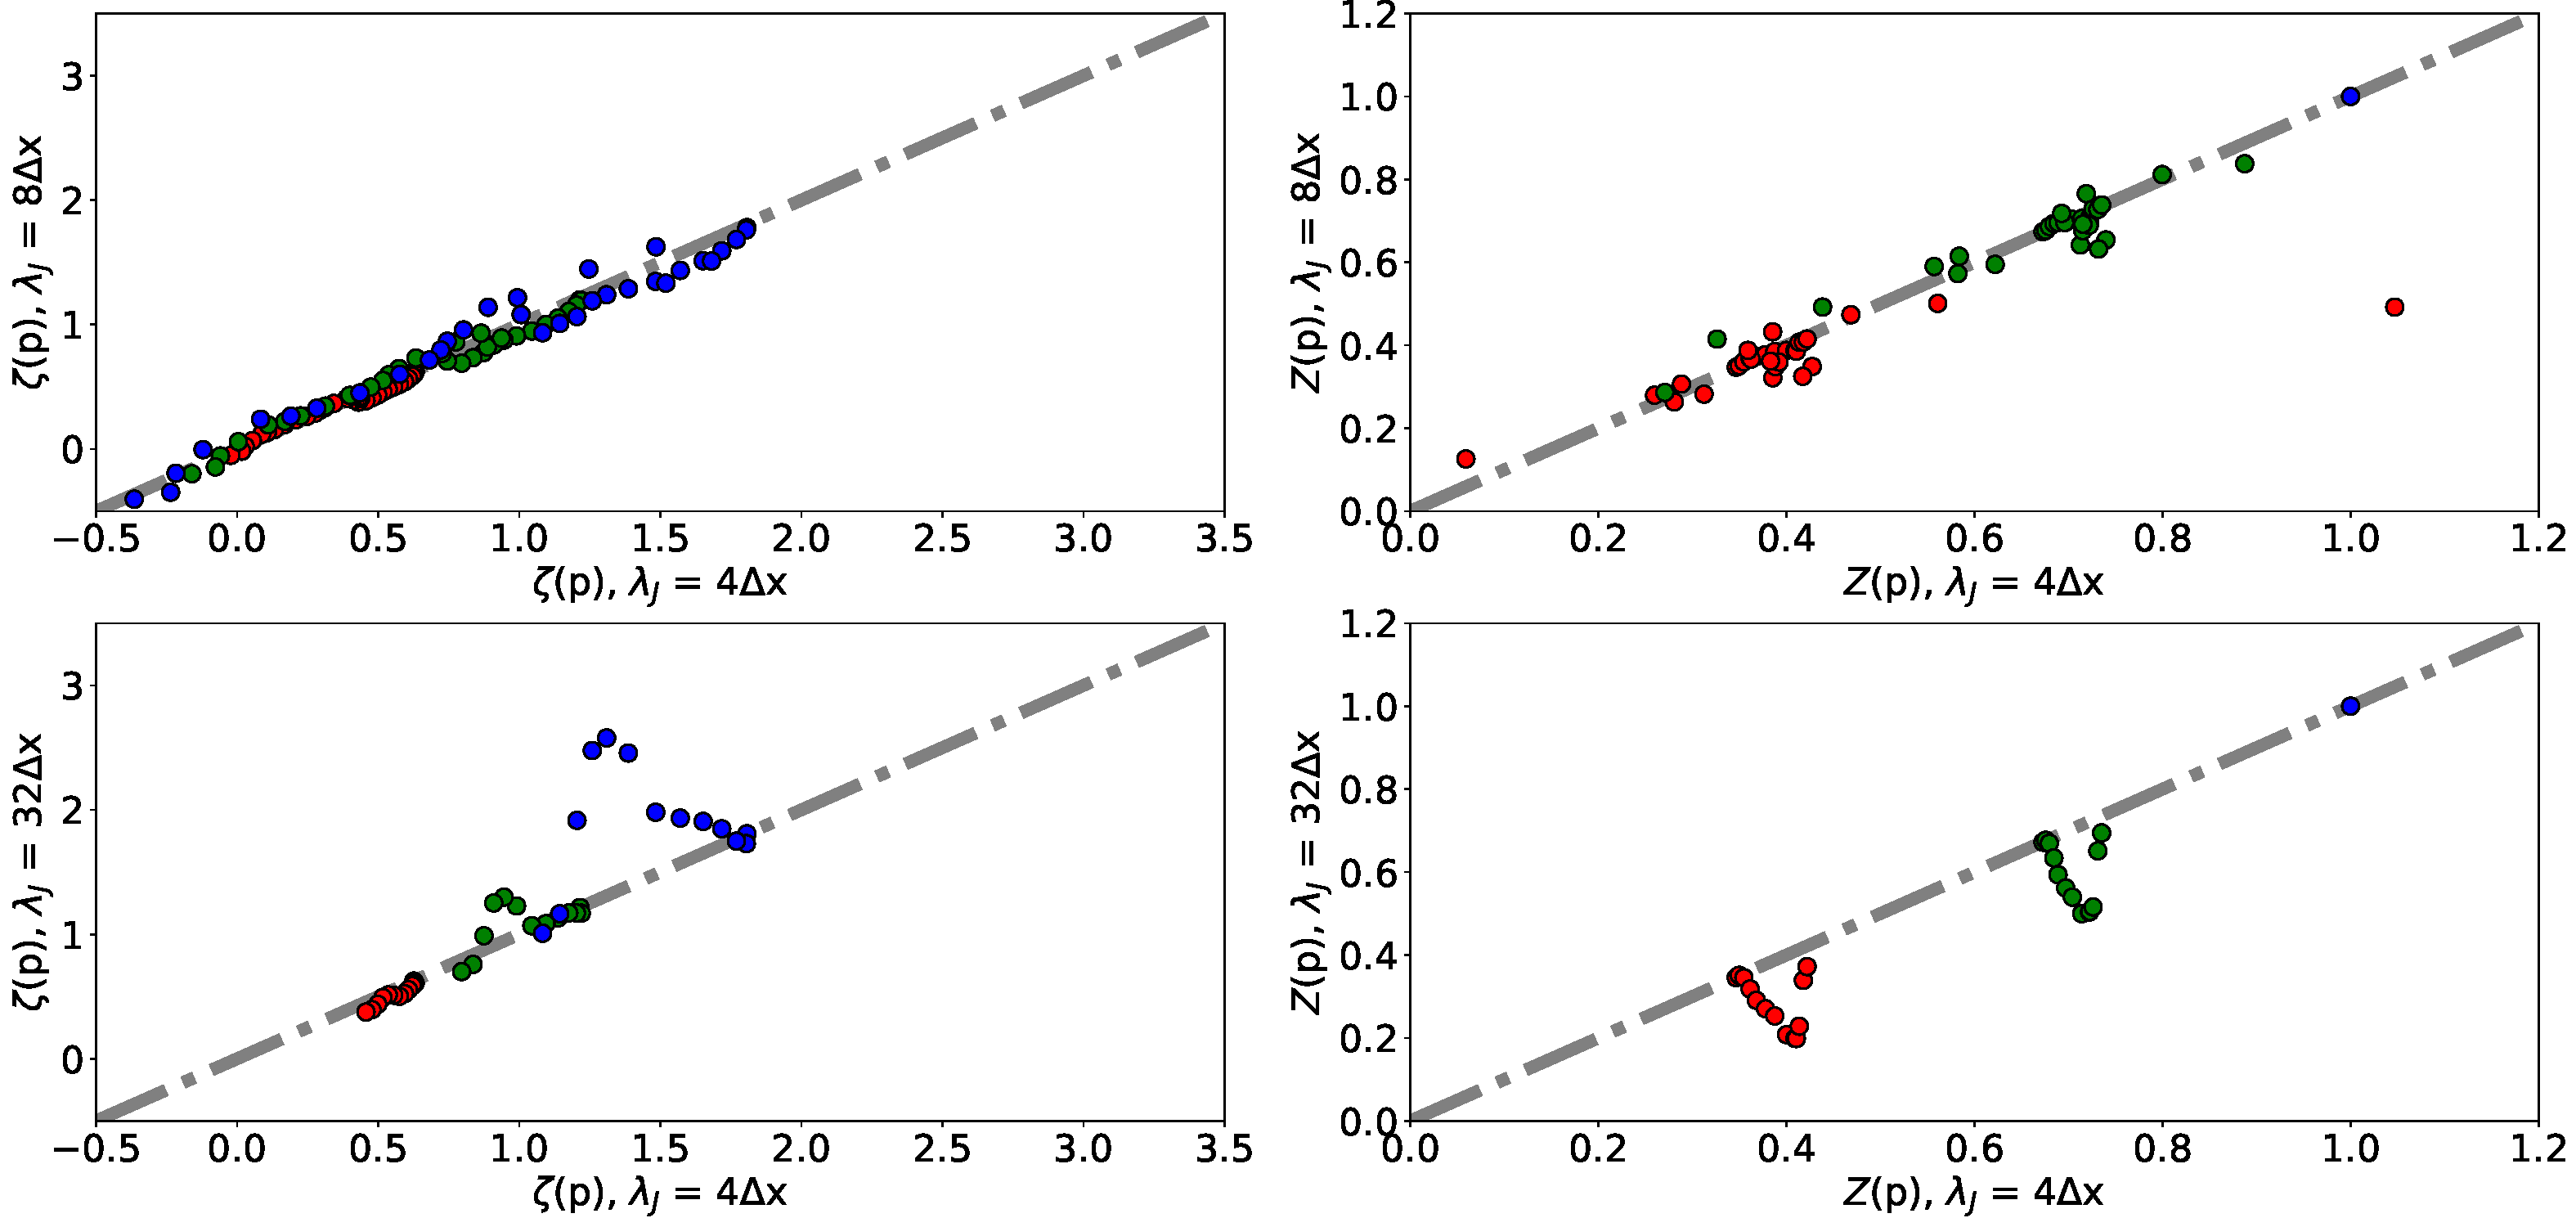
\includegraphics[width=\textwidth]{comp_jeans.pdf}
    \caption{Comparison of measure VSF sclaing exponents, $\zeta$ (\textit{left}), and self-similarity parameters, $Z$ (\textit{right}), depending on the Jeans refinement of the simulation runs the data are based on, respectively. The \textit{abscissas}, thereby, always refers to the measurements based on $\lambda_J$~=~$4\Delta{}x$, while the \textit{ordinates} of the do so the $\lambda_J$~=~$8\Delta{}x$ (\textit{top}) and $\lambda_J$~=~$32\Delta{}x$ (\textit{bottom}) measurements. All data points based on the \texttt{M3} cloud and represent the same time step in the respective simulations. 
    }
    \label{pic:results:jeans_comp}
\end{figure*}

At $t$~=~1.2~Myr, the last time step of this sample, the values of all $\zeta$ equal the measurements of $\lambda_J$~=~$4\Delta{}x$ again.
As there is no information of how the $\lambda_J$~=~$32\Delta{}x$ simulations develop further we cannot predict whether this correspondence will continue. 
